%%%%%%%%%%%%%%%%%%%%%%%%%%%%%%%%%%%%%%%%%%%%%%%%%%%
%
%  New template code for TAMU Theses and Dissertations starting Fall 2012.
%  For more info about this template or the
%  TAMU LaTeX User's Group, see http://www.howdy.me/.
%
%  Author: Wendy Lynn Turner
%	 Version 1.0
%  Last updated 8/5/2012
%
%%%%%%%%%%%%%%%%%%%%%%%%%%%%%%%%%%%%%%%%%%%%%%%%%%%

%%%%%%%%%%%%%%%%%%%%%%%%%%%%%%%%%%%%%%%%%%%%%%%%%%%%%%%%%%%%%%%%%%%%%%
%%                           SECTION I
%%%%%%%%%%%%%%%%%%%%%%%%%%%%%%%%%%%%%%%%%%%%%%%%%%%%%%%%%%%%%%%%%%%%%


\pagestyle{plain} % No headers, just page numbers
\pagenumbering{arabic} % Arabic numerals
\setcounter{page}{1}


\chapter{\uppercase {Background: The Image Synthesis Process}}

3D Rendering can be described as the process of creating 2D images from 3D geometric shapes with the use of photorealistic/nonphotorealistic effects on a computer. For this thesis the process of image synthesis has been broken into four milestones.  Ray casting and ray tracing will also be described as the process of generating an image by tracing the path of virtual rays from an eye source through pixels in an image plane and simulating the effects of its encounters with virtual objects.  Each will be differentiated further by their illumination models, which is the shading algorithms used to interact with light rays. Out of the four milestones for this thesis, three are associated directly with image synthesis theory: direct illumination, distributed ray tracing, and indirect illumination.

\section{Direct Illumination: Ray Casting}

A landscape figure should be shown below.
%%%%%%%%%%%%%%%%%%%%%%%%%%%%%%%%%%%%%%%%%%%%%%%%%%%%%%
\begin{sidewaysfigure}[H]
\centering
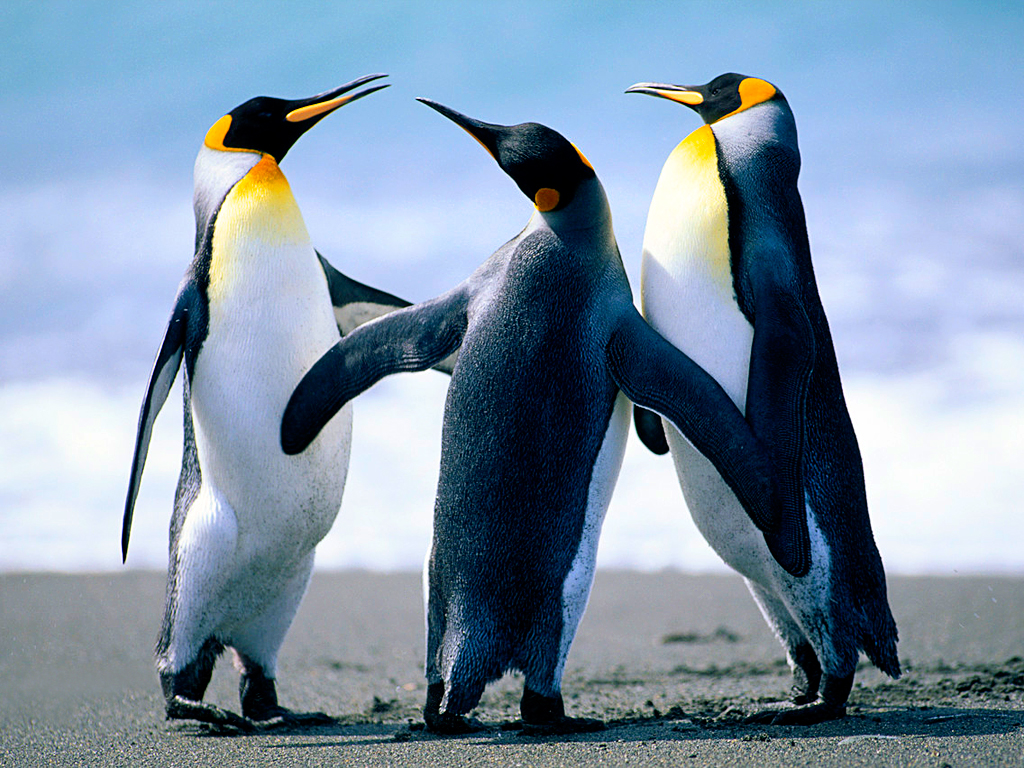
\includegraphics[scale=.50]{figures/Penguins.jpg}
\caption{TAMU figure - This is an example of a long figure title with a landscape figure.  Figure titles need to be single-spaced within and double spaced between in the list of figures.}
\label{fig:tamu-fig1-1}
\end{sidewaysfigure}
%%%%%%%%%%%%%%%%%%%%%%%%%%%%%%%%%%%%%%%%%%%%%%%%%%%%%%

More text here goes here.


Lorem ipsum dolor sit amet, consectetur adipiscing elit. Morbi augue urna, varius quis facilisis ac, imperdiet et nunc. Vestibulum ante ipsum primis in faucibus.

\section{Ray Tracing and Distributed Ray Tracing}
Maecenas accumsan lobortis dui fringilla suscipit. Quisque congue fringilla dui, sed eleifend sapien fringilla euismod. Pellentesque habitant morbi tristique senectus et netus et malesuada fames ac turpis egestas. Maecenas venenatis posuere magna quis tempus. Cras at leo massa, eu ultricies tellus. Nunc nec dictum augue. Cum sociis natoque penatibus et magnis dis parturient montes, nascetur ridiculus mus. Phasellus purus felis, mollis id scelerisque in, viverra in elit. Nulla iaculis ultrices justo, ac pharetra nisl rhoncus pulvinar. Duis vitae mauris velit, in congue massa.

Donec lectus orci, bibendum ut blandit dignissim, molestie non eros. Praesent aliquet feugiat dignissim. Morbi porttitor sollicitudin nisl, non mollis quam ultrices sit amet. Cras feugiat lacinia diam ut convallis. Nam nec varius ante. Nunc a ultrices felis. Quisque luctus sapien et ligula ornare quis consequat urna aliquet. Vestibulum vulputate lorem a tellus auctor id commodo risus sodales. Suspendisse quis tortor a felis molestie laoreet ut a nunc. Donec gravida sapien eget mauris condimentum lacinia. Proin eu purus libero. Nullam augue mi, vestibulum in convallis eu, adipiscing ac arcu. Donec nisi libero, egestas et molestie in, mollis quis ipsum. Sed gravida quam sit amet ante tempus rutrum non in mi. Cras viverra facilisis eros, id vestibulum sapien malesuada eget. Maecenas imperdiet luctus nisi vitae suscipit.



Aliquam erat volutpat. Integer ut mauris elit. Nam et lectus vel neque vehicula commodo. Integer at risus ligula. Fusce mollis mauris sed lorem aliquam bibendum porttitor tellus blandit. Curabitur enim nibh, accumsan eu elementum id, rutrum a ipsum. Vivamus ultricies, elit id ornare iaculis, metus justo posuere quam, sit amet bibendum arcu dolor a eros. Sed in nisl nibh. Aenean egestas est ut tortor volutpat vehicula. Maecenas aliquet placerat nunc hendrerit dictum. In et nisi massa. Pellentesque luctus, sapien quis dignissim vulputate, sapien libero bibendum velit, vitae auctor ipsum nulla at augue. Nulla ac eros vitae tortor elementum vehicula.

Morbi tristique egestas placerat. Cras faucibus eleifend porta. Class aptent taciti sociosqu ad litora torquent per conubia nostra, per inceptos himenaeos. Ut a pellentesque neque. Donec sollicitudin metus varius nulla egestas laoreet. Duis non mauris ut nunc adipiscing volutpat. Nam vitae est sed turpis tristique varius.

\subsection{This is a Very Long Subsection Title This is a Very Long Subsection Title}

More text
\subsection{Subsection}

Subsection text

\section{Indirect Illumination}

Section text
